\section{Ergebnisse und Berechnungen}
\label{sec:ergebnisse}
\subsection{Versuchteil 1:}
 
 %Start
 \begin{figure}[h!]
 	\centering
 	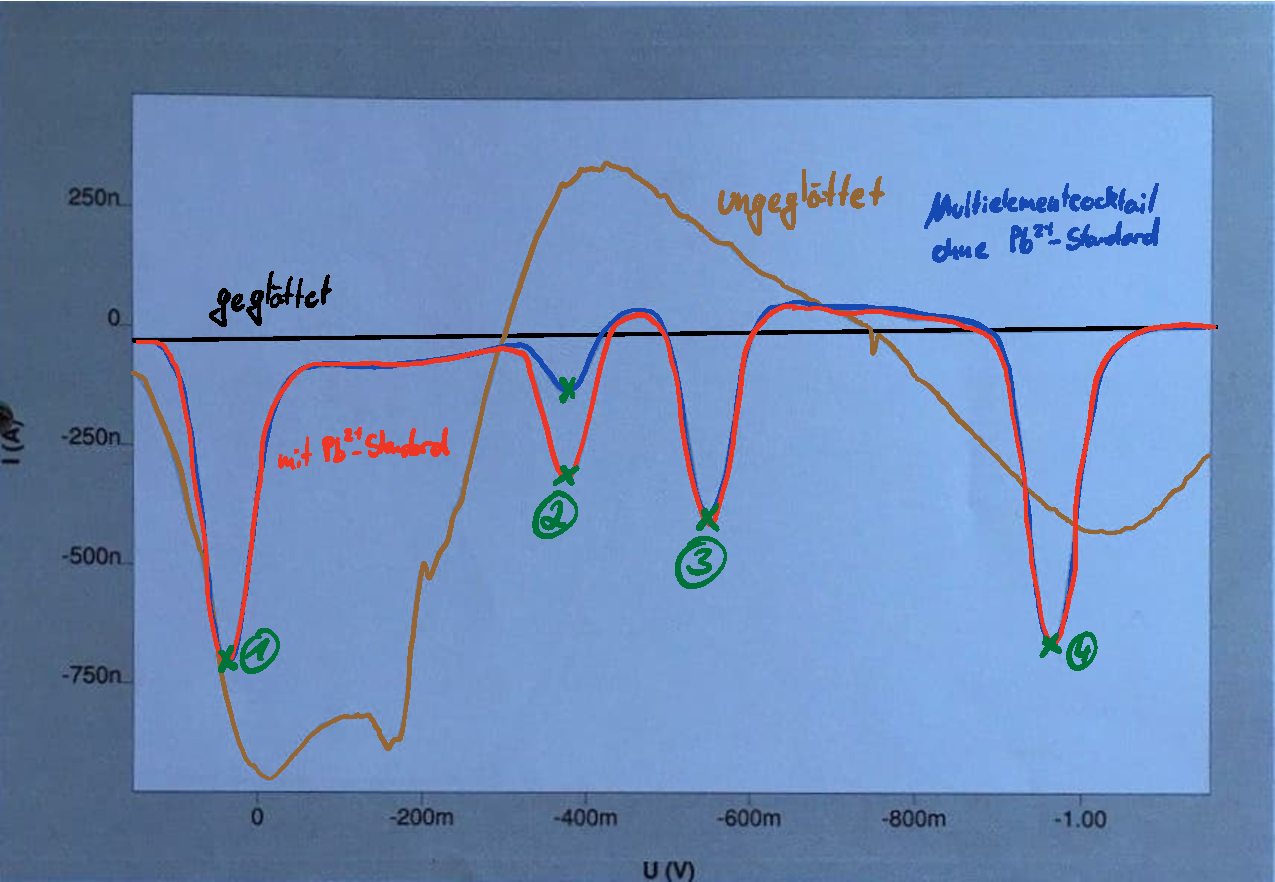
\includegraphics[width=0.9\textwidth]{img/Daten_farbig2}
 	\caption{Strom-Spannungskurven (Polarogramme) des Versuchsteils 1}
 	\label{fig:daten_farbig}
 \end{figure}
 \FloatBarrier
 %Ende     
 %Tabelle START
 \vspace*{-2.5mm}
 \renewcommand{\arraystretch}{1.2}
 \begin{table}[h!]
 	\centering
 	\caption{Zuordnung der Peaks den Elementen des Multielementencocktails}
 	\label{tab:peaks}
 %	\resizebox{17cm}{!}{
 	\begin{tabulary}{\textwidth}{C|C|C|C|C}
 		\hline
 		\textbf{Element} &  \textbf{Kupfer}  &\textbf{Blei}& \textbf{Cadmium} & \textbf{Zink}\\ 
 	&\ce{Cu}&\ce{Pb}&\ce{Cd}&\ce{Zn}\\
 		\hline
 		\textbf{Peak} &1&2&3&4\\
 		\hline
 		\textbf{Std.-Elektrodenpotential [V]}&$+0,52$&$-0,13$&$-0,40$&$-0,76$\\
 		\hline
 	\end{tabulary}
 	%}
 \end{table}
 \FloatBarrier
 \vspace*{-2.5mm}
 %Tabelle ENDE
 
 
\newpage
 
 \subsection{Versuchsteil 2:}

	\textcolor{red}{Polarogramm Probe mit Aufstockungen ?}\\
	\textcolor{red}{Quantitative Auswertung des Programms}
	
	\subsubsection*{	Berechnung der Blei-Standard-Zugaben-Konzentration:}
	\begin{flalign}\label{gl:7}
	V_{\text{Standard-Zugabe}} * c_{\text{Standard-Zugabe}} &= V_{\text{Lösung}} * c_{\text{Lösung}}\\
	c_{\text{Lösung}} 	&= \frac{V_{\text{Standard-Zugabe}} }{V_{\text{Lösung}}} * c_{\text{Standard-Zugabe}}		
	\end{flalign}
	\begin{flalign}\label{gl:8}
	c_{\text{Lösung},1} &=\frac{\SI{200e-6}{\liter}}{\SI{25e-3}{\liter}} * \SI{1000}{\milli \gram \per \liter}\\
	&= \underline{\SI{8}{\milli \gram \per \liter}	}\\[3mm]
	c_{\text{Lösung},2} &=\frac{\SI{400e-6}{\liter}}{\SI{25e-3}{\liter}} * \SI{1000}{\milli \gram \per \liter}\\
	&= \underline{\SI{16}{\milli \gram \per \liter}	}
	\end{flalign}
	
	
	 %Tabelle START
	\vspace*{-2.5mm}
	\renewcommand{\arraystretch}{1.2}
	\begin{table}[h!]
		\centering
		\caption{Messwerte der Messreihe 1}
		\label{tab:messreihe1}
		%\resizebox{10cm}{!}{
		\begin{tabulary}{\textwidth}{C|CC}
			\hline
			\textbf{Konzentration der Bleizugabe in \si{\milli \gram \per \liter}} &  \textbf{Spannung in \si{\volt}}  &\textbf{Stromstärke in \si{\nano \ampere}}\\ 
			\hline
			0 	&-0,376	&-113,0	\\
			0 	&-0,376	&-112,5	\\
			8 	&-0,376	&-268,2	\\
			8 	&-0,376	&-266,6	\\
			16 	&-0,376	&-422,8	\\
			16 	&-0,382	&-416,0	\\
			\hline
		\end{tabulary}
		%}
	\end{table}
	\FloatBarrier
	\vspace*{-2.5mm}
	%Tabelle ENDE
	%Tabelle START
	\vspace*{-2.5mm}
	\renewcommand{\arraystretch}{1.2}
	\begin{table}[h!]
		\centering
		\caption{Messwerte der Messreihe 2}
		\label{tab:messreihe2}
		%\resizebox{10cm}{!}{
		\begin{tabulary}{\textwidth}{C|CC}
			\hline
			\textbf{Konzentration der Bleizugabe in \si{\milli \gram \per \liter}} &  \textbf{Spannung in \si{\volt}}  &\textbf{Stromstärke in \si{\nano \ampere}}\\ 
			\hline
			0 	&-0,382	&-129,3	\\
			0 	&-0,382	&-139,2	\\
			8 	&-0,382	&-286,2	\\
			8 	&-0,382	&-282,2	\\
			16 	&-0,382	&-425,1	\\
			16 	&-0,382	&-424,0	\\
			\hline
		\end{tabulary}
		%}
	\end{table}
	\FloatBarrier
	\vspace*{-2.5mm}
	%Tabelle ENDE
	
	\pagebreak

	\subsubsection*{Aufstellen der Kalibriergeraden:}
	Die Kalibriergerade wird manuell erstellt in dem die die gemessenen Stromstärken der Peaks über dem Konzentrationszuschuss durch die Zugabe der Blei Standardlösung aufgetragen werden. Die Stromstärken für die Y-Achse werden aus den gewonnenen Polarogrammen abgelesen. Hier treten Ablesefehler von etwa $\pm$ \SI{10}{\nano\ampere} auf. Die Konzentrationsänderung bei Addition von Standardlösung wird entsprechend der Gleichungen (\ref{gl:7}) und (\ref{gl:8}) berechnet. Mittels des Tabellenkalkulationsprogramms \textit{LibreOffice Calc} wurde eine lineare Regression zur Bestimmung der Kalibriergeradengleichung durchgeführt. Es ergaben sich folgende Funktionsgleichungen:
	$$f_1(x)=y=-19,166*x - 113,19 $$ 
	$$f_2(x)=y=-18,144*x - 135,85 $$ 
	
	\begin{figure}[h!]
		\begin{center}
			\resizebox{0.9\textwidth}{!}{
				\begin{tikzpicture}[trim axis left, trim axis right]
				\begin{axis}[
				axis lines = middle,
				width = 20cm,
				height = 11cm,
				xmin = -10,
				xmax = 20,
				%	ymin = -0.1,
				%	ymax = 0,
				%	ytick = {-4.5,-4,...,-1},
				xtick = {-10,-9,...,20},
				ylabel={Stromstärke in \si{\nano \ampere}},
				y label style={at={(0.25,0.40)}, rotate=90},
				xlabel={Konzentration der Blei-Standard-Zugabe in \si{\milli \gram \per \milli \liter}},
				legend style={at={(0.75,0.45)},anchor=west},
				y dir = reverse,
				]
				\addplot table {datenm1.dat};
				\addplot +[mark=none, dashed, black, domain=-10:20] {-19.166*x - 113.19};
				\addplot table {datenm2.dat};
				\addplot +[mark=none, dotted, black, domain=-10:20] {-18.144*x - 135.85};
				
				\legend{Messreihe 1, Regression Messreihe 1,Messreihe 2, Regression Messreihe 2};
				\end{axis}
				\end{tikzpicture}
			}
			\caption{Berechnete Leitungen in Abhängigkeit von der Konzentration der Blei-Standardzugabe (siehe Tab. \ref{tab:messreihe1} und Tab. \ref{tab:messreihe2})}
			\label{dia:lnr/lnc}
		\end{center}
	\end{figure}
	\FloatBarrier
	\vspace*{-5mm}
	
%	\begin{figure}[h!]
%		\begin{center}
%			\resizebox{0.8\textwidth}{!}{
%				\begin{tikzpicture}[trim axis left, trim axis right]
%				\begin{axis}[
%				axis lines = left,
%				width = 13cm,
%				height = 7cm,
%				xmin = -9,
%				xmax = 17,
%				ymin = 0,
%				ymax = 450,
%				%ytick = {0,2,...,14},
%				%xtick = {0,10,...,100},
%				ylabel={Stromstärke I [\si{\nano\ampere}]},
%				xlabel={Zugesetzte Bleikonzentration [\si{\milli\gram\per\liter}]},
%					legend style={at={(0.5,0.95)},anchor=west},
%				scatter/classes={
%					a={mark=square*,blue},
%					b={mark=triangle*,red},
%					c={mark=o,draw=black}
%				}
%				]
%%				\addplot[scatter,only marks,
%%				scatter src=explicit symbolic]
%%				coordinates {
%%					(0,125) 	[a]
%%					(8,275) 	[a]
%%					(16,429.1662)[a]
%%					(0,141.667) 	[b]
%%					(8,291.667)    	[b]
%%					(16,429.1667)	[b]
%%				};
%				\addplot[blue,domain=-8:16]{19.01041875*x+124.30555};
%				\addplot[red,domain=-8:16]{17.96872125*x+143.75038333};
%				\legend{Messreihe 1,Messreihe 2};
%				\end{axis}
%				\end{tikzpicture}
%			}
%			\caption{Kalibriergeraden - manuell}
%			\label{dia:kalibriergeraden}
%		\end{center}
%	\end{figure}
%	\FloatBarrier
	Die Nullstellen der Kalibriergeraden liegen bei -5,906 und -7,487. Der Betrag dieser Werte entspricht der Ausgangskonzentration von \SI{5,906}{\milli\gram\per\liter} und \SI{7,487}{\milli\gram\per\liter}. 
	Die manuell ermittelten Konzentrationen entsprechen beinahe den computerberechneten Werten.	\\
	
	\textcolor{red}{--> Stark unterschiedliche Messwerte, Neue Betrachtung nötig}
	
	\pagebreak
	
	\subsubsection*{Ausreißertests der zusammengefassten Messreihen 1 und 2:}
	
	\textbf{Berechnung des Mittelwertes:}
	\begin{flalign}\label{Gl:Mittelwert-Beispielrechnung1}
		\bar{x} &= \frac{\sum_{n=1}^{N}x_n}{N}
	\end{flalign}
	\begin{flalign}\label{Gl:Mittelwert-Beispielrechnung2}
	\bar{x} &= \frac{-139,2-129,2-113,0-112,5}{4}
			&= \underline{-123,5}
	\end{flalign}
	
	\textbf{Berechnung der Standardabweichung:}
	\begin{flalign}\label{Gl:Standardabweichung-Beispielrechnung}
	s &= \sqrt{\frac{\sum_{n=1}^{N}(x_n-\bar{x})^2}{N-1}}
	\end{flalign}
%	\begin{footnotesize}
		\begin{flalign}
		s &= \sqrt{\frac{(-139,2+123,5)^2+(-129,3+123,5)^2+(-113,0+123,5)^2+(-112,5+123,5)^2}{3}}\\
		&= \underline{11,3}
		\end{flalign}
%	\end{footnotesize}
	

	
	\textbf{Berechnung des Q-Wertes:}
	\begin{flalign}
		Q_{\text{emp}} &= \frac{x_{n+1}-x_n}{x_n-x_1}
	\end{flalign}
	\begin{flalign}
		Q_{\text{emp}} 	&= \frac{-129,3-(-139,2)}{-112,5-(-139,2)}\\
						&= \underline{0,371}\\[2mm]
		Q_{\text{tab}}	&> Q_{\text{emp}} \rightarrow\text{Kein Ausreißer}\\
		0,829			&> 0,371 \rightarrow \underline{\text{Kein Ausreißer}: \text{wahr}}
	\end{flalign}
	
	\textbf{Berechnung des G-Wertes:}
	\begin{flalign}
	G_{\text{emp}} &= \frac{|x_{\text{Test}}-\bar{x}|}{s}
	\end{flalign}
	\begin{flalign}
	G_{\text{emp}} 	&= \frac{|-139,2-(-123,5)|}{11,3}\\
	&= \underline{1,389}\\[2mm]
	G_{\text{tab}}	&> G_{\text{emp}} \rightarrow\text{Kein Ausreißer}\\
	1,463			&> 1,389 \rightarrow \underline{\text{Kein Ausreißer}: \text{wahr}}
	\end{flalign}
	
	%Tabelle START
	\vspace*{-2.5mm}
	\renewcommand{\arraystretch}{1.2}
	\begin{table}[h!]
		\centering
		\caption{Zusammengefasste, aufsteigend sortierte Messwerte mit Mittelwerten und Standardabweichungen}
		\label{tab:Messreihen}
		\resizebox{15cm}{!}{
		\begin{tabulary}{1.3\textwidth}{C|C|C|C}
			\hline
			\textbf{Blei-Standard-Zugabe in \si{\milli \gram \per \liter}}&\textbf{Messwert in \si{\nano \ampere}}&\textbf{Mittelwert}&\textbf{Standardabweichung}\\
			\hline
			\hline
			0&-139,2&&\\
			0&-129,3&-123,5&11,3\\
			0&-113,0&&\\
			0&-112,5&&\\
			\hline
			8&-286,2&&\\
			8&-282,2&-275,8&8,5\\
			8&-268,2&&\\
			8&-266,6&&\\
			\hline
			16&-425,1&&\\
			16&-424,0&-422,0&3,5\\
			16&-422,8&&\\
			16&-416,0&&\\
			\hline
		\end{tabulary}
		}
	\end{table}
	\FloatBarrier
	\vspace*{-2.5mm}
	%Tabelle ENDE	
	
		%Tabelle START
	\vspace*{-2.5mm}
	\renewcommand{\arraystretch}{1.2}
	\begin{table}[h!]
		\centering
		\caption{Zusammengefasste, aufsteigend sortierte Messwerte und empirische Q- und G-Werte zur Ausreißerbewertung}
		\label{tab:Messreihen_ausreisser}
		\resizebox{15cm}{!}{
			\begin{tabulary}{1.4\textwidth}{C|C|C|C|C|C}
				\hline
				\textbf{Blei-Standard-Zugabe in \si{\milli \gram \per \liter}}&\textbf{Messwert in \si{\nano \ampere}}&\textbf{Q-Wert (Tab=0,829)}&\textbf{Q-Ausreißer ?}&\textbf{G-Wert (Tab=1,463)}&\textbf{G-Ausreißer ?}\\
				\hline
				\hline
				0&-139,2&0,371&Nein&1,389&Nein\\
				0&-129,3&-&Nein&0,513&Nein\\
				0&-113,0&-&Nein&0,929&Nein\\
				0&-112,5&0,019&Nein&0,9723&Nein\\
				\hline
				8&-286,2&0,204&Nein&1,218&Nein\\
				8&-282,2&-&Nein&0,750&Nein\\
				8&-268,2&-&Nein&0,890&Nein\\
				8&-266,6&0,082&Nein&1,078&Nein\\
				\hline
				16&-425,1&0,121&Nein&0,882&Nein\\
				16&-424,0&-&Nein&0,571&Nein\\
				16&-422,8&-&Nein&0,233&Nein\\
				\textit{16}&\textit{-416,0}&\textit{0,747}&\textit{Nein}&\textit{1,686}&\textit{Ja}\\
				\hline
			\end{tabulary}
		}
	\end{table}
	\FloatBarrier
	\vspace*{-2.5mm}
	%Tabelle ENDE
	
		\begin{figure}[h!]
		\begin{center}
			\resizebox{0.9\textwidth}{!}{
				\begin{tikzpicture}[trim axis left, trim axis right]
				\begin{axis}[
				axis lines = middle,
				width = 20cm,
				height = 11cm,
				xmin = -10,
				xmax = 20,
				%	ymin = -0.1,
				%	ymax = 0,
				%	ytick = {-4.5,-4,...,-1},
				xtick = {-10,-9,...,20},
				ylabel={Stromstärke in \si{\nano \ampere}},
				y label style={at={(0.25,0.40)}, rotate=90},
				xlabel={Konzentration der Blei-Standard-Zugabe in \si{\milli \gram \per \milli \liter}},
				legend style={at={(0.75,0.45)},anchor=west},
				y dir = reverse,
				]
				\addplot table {datenm3.dat};
				\addplot +[mark=none, dashed, black, domain=-10:20] {-18.792*x - 124.153};
				
				\legend{Messreihen 1+2 (korrigiert), Regression Messreihe 1+2 (korrigiert)};
				\end{axis}
				\end{tikzpicture}
			}
			\caption{Korrigierte Kalibrierkurve der Messreihen 1 und 2}
			\label{dia:kalibrier_neu}
		\end{center}
	\end{figure}
	\FloatBarrier
	\vspace*{-5mm}
	
	
	  %Tabelle START
	  \vspace*{-2.5mm}
	  \renewcommand{\arraystretch}{1.2}
	  \begin{table}[h!]
	  	\centering
	  	\caption{Vergleich der ermittelten Konzentrationen aus manueller und Computergestützter Berechnung}
	  	\label{tab:mauell,automatisch}
	  		\resizebox{15cm}{!}{
	  	\begin{tabulary}{1.3\textwidth}{L|C|C|C||C|C}
	  		\hline
	  		&\textbf{Computer}&\textbf{Manuell einzeln}&\textbf{Manuell}&\textbf{Mittelwert}&\textbf{Standardabweichung}\\
	  		\hline
	  		\hline
		  	$c_1$&\SI{5,757}{\milli\gram\per\liter}&\SI{5,906}{\milli\gram\per\liter}&\SI{6,606}{\milli\gram\per\liter}&&\\
	  		\hline
	  		$c_2$&\SI{7,186}{\milli\gram\per\liter}&\SI{7,487}{\milli\gram\per\liter}&-&&\\
	  		\hline
	  		\hline
	  		$\bar{c}$&\SI{6,472}{\milli\gram\per\liter}&\SI{6,697}{\milli\gram\per\liter}&\SI{6,606}{\milli\gram\per\liter}&\SI{6,591}{\milli \gram \per \liter}&\SI{0,113}{\milli \gram \per \liter}\\
	  		\hline
	  		
	  	\end{tabulary}
	  	}
	  \end{table}
	  \FloatBarrier
	  %Tabelle ENDE
	  
	  \subsubsection*{Bestimmung des Bleigehaltes in der originalen Probe:}
	  
	  \textcolor{red}{Für Vertrauensbereich werden alle drei Auswertungsmethoden heran gezogen. Ist das so richtig gedacht ?}\\
	  \textcolor{blue}{Ja, ich denke das ist die sinnvollste Variante und am Aussagekräftigsten.}
	  \textbf{Berechnung des Vertrauensintervalls:}\\
	  Für die Berechnungen des Mittelwertes und der Standardabweichung siehe Gl. (\ref{Gl:Mittelwert-Beispielrechnung1}),(\ref{Gl:Mittelwert-Beispielrechnung2}) und (\ref{Gl:Standardabweichung-Beispielrechnung}).
	  \begin{flalign}
	  	conf(\bar{x}) 	&= \bar{x}\pm \frac{t}{\sqrt{N}}*s				
	  \end{flalign}
	   \begin{flalign}
	  	conf(\bar{x})	&= \SI{6,591}{\milli \gram \per \liter}\pm \frac{4,303}{\sqrt{3}}*\SI{0,113}{\milli \gram \per \liter}\\
	  					&= \underline{\SI{6,591}{\milli \gram \per \liter}\pm \SI{0,280}{\milli \gram \per \liter}}
	  \end{flalign}
	  
	  
	  	
	
	\subsubsection*{Aliquotierfaktor:} 
	Der Aliquotierfaktor dient zur Hochrechnung auf das gesamte Probenvolumen. Die Bleihaltige Probe wurde zuvor auf \SI{100}{\milli\liter} aufgefüllt, wovon jeweils \SI{25}{\milli\liter} in das Messgerät gegeben wurden. Das Ergibt nach Gl.\ref{gl:aliquo} einen Aliquotierfaktor von 4.
	\begin{equation}\label{gl:aliquo}
		f_A=\frac{\SI{100}{\milli\liter}}{\SI{25}{\milli\liter}}=4
	\end{equation}
	
	\textbf{Berechnung der Masse der Originalprobe:}
	\begin{flalign}
		m_{\text{original}} &= m_{\text{mess}} *f_A\\
		m_{\text{original}} &= V_{\text{mess}} *c*f_A
	\end{flalign}
	\begin{flalign}
	m_{\text{original}} 	&= m_{\text{mess}} *f_A\\
	m_{\text{original}} 	&= V_{\text{mess}} *c*f_A\\
							&= \SI{25e-3}{\liter} *\left(\SI{6,591}{\milli \gram \per \liter}\pm \SI{0,280}{\milli \gram \per \liter}\right)*4\\
	m_{\text{original}} 	&=\SI{0,659}{\milli \gram}\pm \SI{0,0280}{\milli \gram}
	 = \underline{\SI{659,1}{\micro \gram}\pm \SI{28,0}{\micro \gram}}\\
	\end{flalign}


\pagebreak

